\documentclass{beamer}
%\mode<presentation>{\usepackage{beamerthemesplit}}

%\usepackage{beamerthemebars}
\usepackage{amsmath}
\renewcommand{\baselinestretch}{1.2}
\usepackage{cite}
\usepackage{url}
\usepackage{longtable}
%\usepackage[dvips]{graphicx,color}
%\usepackage{makeidx}
\usepackage{nomencl}
\usepackage{amssymb}
%\usepackage{psfig}
%\usepackage{epsfig}
\usepackage{graphicx}
\usepackage{amssymb}
\usepackage{multicol}
\usepackage[bottom]{footmisc}
\usepackage{subfigure}
\usepackage[OT2,OT1]{fontenc}
\newcommand{\imsize}{3in}

\useinnertheme{rounded}
\usecolortheme{whale}
%\usecolortheme{orchid}
\useoutertheme{infolines}
%\useoutertheme{shadow}

%change your title
\title{Semiconductor Based Gas Sensors }
\subtitle{Special Topic Seminar}
%\institute{\normalsize{IIT Bombay}}
%\setbeamercolor{title}{fg=white,bg=black}

\begin{document}
\author[SysCon] {By \\ \vspace{0.05in} \textbf{Yogesh M. Gulekar } \\ \vspace{0.01in} {Under the Guidance of} \\ \textbf{Prof. M. D. Patil}\\
\textcolor{black}{ \\ Department of Electronics Engineering} \\ \textcolor{black}{Ramrao Adik Institute of Technology,\\ Nerul, Navi Mumbai } \\
}

\begin{frame}
\begin{center}
\end{center}
\titlepage
\end{frame}

%Slide which includes bullated items
\begin{frame}
\frametitle{Motivation}
\begin{itemize}
\item {The existing gas sensors are having many limitations.}
\item {Many types of sensors are available in market but semiconductor based gas sensors are widely used for their various applications.}
\item {The semiconductor based gas sensors have more features than primitive gas sensors.}
\item {They can also be categorized by the type of gas they detect}
\end{itemize}
\end{frame}


%Slide which includes bullated items having numerical no.
\begin{frame}
\frametitle{Outline}
\begin{enumerate}
\item {Introduction}
\item {Brief explanation of existing gas sensors}
\item {Limitations of existing gas sensors }
\item {Advantages of semiconductor based gas sensors}
\item {Applications}
\end{enumerate}
\end{frame}

%Slide which includes bullated items having numerical no.
\begin{frame}
\frametitle{Introduction to gas sensors(IR Gas Sensor)}
The essential components of an IR system are:\newline
 Source of IR radiation.\newline
Detector capable of seeing the IR radiation.\newline
Path between the detector and the source open to the gas to be detected.\newline

Principle:\newline
The detector measures the difference between the dark (no light hitting the detector)
and light (full energy hitting the detector)
\end{frame}

%Slide which includes figure
\begin{frame}
\frametitle{Introduction to gas sensors} Schematic of
Infra Red Sensors
\begin{figure}[tbh]
\begin{center}
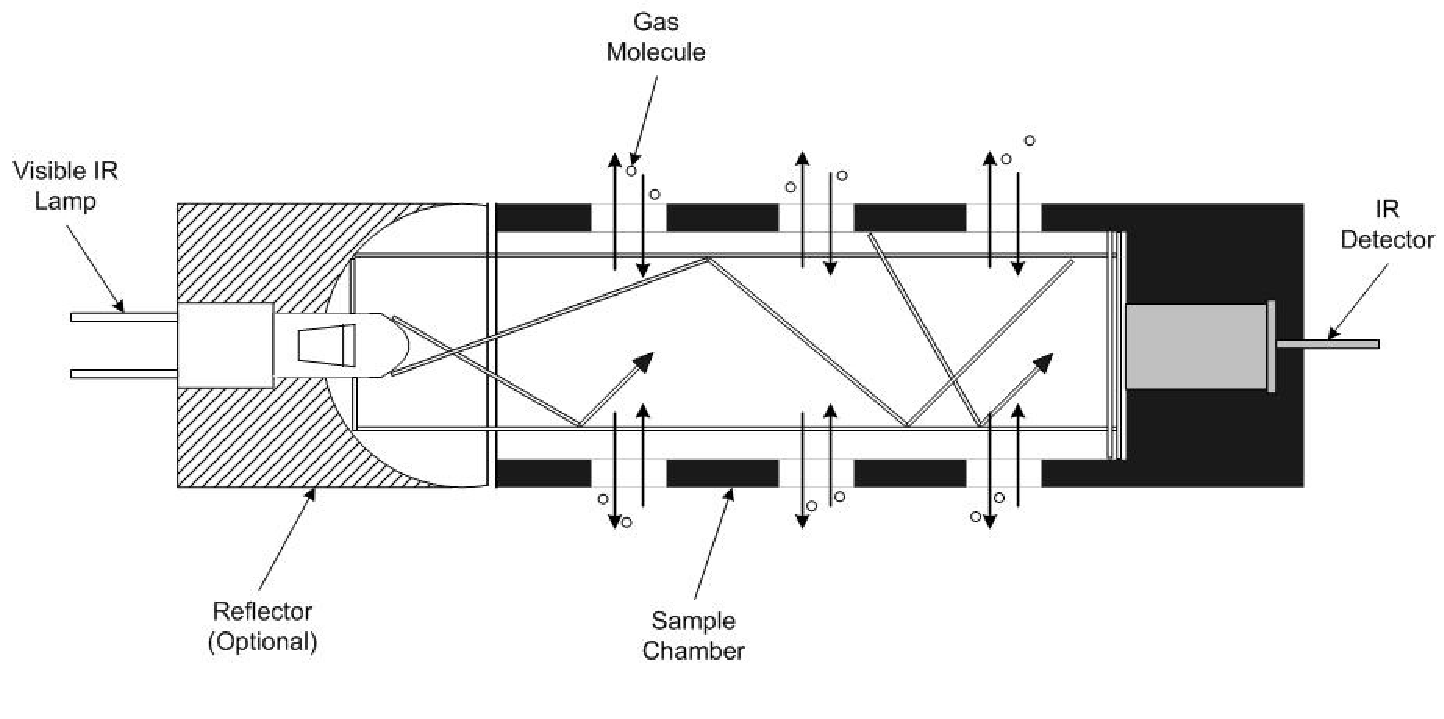
\includegraphics[width= 4 in]{IR.pdf}
\end{center}
%\caption{The two degree-of-freedom structure in QFT} \label{tdof}
\end{figure}
\end{frame}

%Slide which includes bullated items having numerical no.
\begin{frame}
\frametitle{Limitations}
\begin{itemize}
\item They are not sensitive (need high concentration or long paths)
  \item They are expensive.
  \item They are not portable.
  \item They cannot monitor all gases (only nonlinear molecules)
  \item They can be affected by humidity and water.
  \item They can be expensive and dust and dirt can coat the optics and impair response.\newline
\end{itemize}
\end{frame}


%Slide which includes bullated items having numerical no.
\begin{frame}
\frametitle{Semiconductor Principle}
The semiconductor gas sensor is composed of:\newline
Sensing element.\newline
Sensor base.\newline
Sensor cap.\newline

Principle:\newline
When a metal oxide crystal is heated at a certain high temperature in air, oxygen is adsorbed on the crystal surface with a negative charge. A surface potential is formed to serve as a potential barrier against electron-flow which is nothing but the electrical resistance of the sensor material.
\end{frame}

%Slide which includes figure
\begin{frame}
\frametitle{Semiconductor Principle}
%\begin{figure}[tbh]
%\begin{center}
%\includegraphics[width= 4 in]{semiconductor.pdf}
%\end{center}
%%\caption{The two degree-of-freedom structure in QFT} \label{tdof}
%\end{figure}
\end{frame}

%Slide which includes figure
\begin{frame}
\frametitle{Semiconductor Principle}
%\begin{figure}[tbh]
%\begin{center}
%\includegraphics[width= 4 in]{principle1.pdf}
%\end{center}
%%\caption{The two degree-of-freedom structure in QFT} \label{tdof}
%\end{figure}
\end{frame}

\begin{frame}
\frametitle{Relationship}
\begin{equation}\label{1}
R_{s} = A[C^{-\alpha}]
\end{equation}\newline
Where: $R_{s}$ = electrical resistance of the sensor\newline
A = constant\newline
[C] = gas concentration\newline
$\alpha$ = slope of Rs curve
\newline

Due to the logarithmic relationship between sensor resistance and gas concentration, semiconductor type sensors have an advantage of high sensitivity to gas even at low gas concentration.
\end{frame}

%Slide which includes figure
\begin{frame}
\frametitle{Applications of Semiconductor based gas sensors}Tungsten-Based SOI Microhotplates for Smart Gas Sensors:\newline

Tungsten-based micro gas sensors overcome problems like high cost and high power consumption.\newline
The small size helps in achieving low power consumption, while the use of existing microelectronics technology can greatly reduce manufacturing costs.
\end{frame}

%Slide which includes figure
\begin{frame}
\frametitle{Applications of Semiconductor based gas sensors}Tungsten-Based SOI Microhotplates for Smart Gas Sensors
%\begin{figure}[tbh]
%\begin{center}
%\includegraphics[width= 4 in]{design.pdf}
%\end{center}
%%\caption{The two degree-of-freedom structure in QFT} \label{tdof}
%\end{figure}
\end{frame}

%Slide which includes figure
\begin{frame}
\frametitle{Applications of Semiconductor based gas sensors}Long-term reliability:\newline

The initial tests carried of the long-term reliability of the microhotplates.\newline
Operating at high temperatures for up to $500^{0}$C.\newline
The results during the operation of the large heater at $350^{0}$C.\newline
The heater  resistance at this temperature is $180^{0}$C, and it required a current of 10 mA.\newline
At this temperature, the tungsten heaters are extremely stable, with a drift of less than 0.1percent

\end{frame}

%Slide which includes figure
\begin{frame}
\frametitle{Applications of Semiconductor based gas sensors}Long-term reliability
%\begin{figure}[tbh]
%\begin{center}
%\includegraphics[width= 4 in]{reliability.pdf}
%\end{center}
%%\caption{The two degree-of-freedom structure in QFT} \label{tdof}
%\end{figure}
\end{frame}

%Slide which includes bullated items having numerical no.
\begin{frame}
\frametitle{Based on PSoC Smart Sensor of Gas Leakage}
\begin{enumerate}
\item {Introduction}
\item {Principle of Acting}
\item {Measurement Circuit }
\end{enumerate}
\end{frame}

%Slide which includes figure
\begin{frame}
\frametitle{Principle of Acting}

A gas sensitive element of the sensor is MEMS technology designed.\newline
It is calibrated and sends a warning message if the gas concentration in air reaches the level of dangerous concentration.\newline
It ensures high reliability and operating life of the device. \newline
The Sensor is made practically on one microcircuit with digital interface due to use PSoC. \newline
It provides high accuracy and low prime cost of the device as a whole.
\end{frame}

%Slide which includes figure
\begin{frame}
\frametitle{Based on PSoC Smart Sensor of Gas Leakage}Block diagram of smart sensor.
%\begin{figure}[tbh]
%\begin{center}
%\includegraphics[width= 1.4 in]{PSOC.pdf}
%\end{center}
%%\caption{The two degree-of-freedom structure in QFT} \label{tdof}
%\end{figure}
\end{frame}

%Slide which includes bullated items having numerical no.
\begin{frame}
\frametitle{Development of a Wireless Integrated Toxic and Explosive MEMS Based Gas Sensor}
\begin{itemize}
\item {Overall System}
\item {Transmitter Module}
\item {Receiver Module }
\end{itemize}
\end{frame}

%Slide which includes figure
\begin{frame}
\frametitle{Overall System}Block Diagram of Overall System.
%\begin{figure}[tbh]
%\begin{center}
%\includegraphics[width= 3 in]{system.pdf}
%\end{center}
%%\caption{The two degree-of-freedom structure in QFT} \label{tdof}
%\end{figure}
\end{frame}

%Slide which includes figure
\begin{frame}
\frametitle{Transmitter Module}Block Diagram of Transmitter.
%\begin{figure}[tbh]
%\begin{center}
%\includegraphics[width= 3 in]{transmitter.pdf}
%\end{center}
%%\caption{The two degree-of-freedom structure in QFT} \label{tdof}
%\end{figure}
\end{frame}

%Slide which includes figure
\begin{frame}
\frametitle{Working Principle}

Change in the concentration produces a change in the resistance and a constant current source is used which provides constant current that flows through this changing resistance.\newline
Voltage changes across the resistance with reference to the change in concentration.\newline
This changing voltage is provided as a input to the voltage controlled oscillator, the output of this VCO is the variation is frequency which in turn related to  change in the concentration.\newline
Concentration is converted accordingly in the frequency variations. As these frequency variations are of low power the RF buffer provides a sufficient gain to these oscillations so that they can be successfully transmitted to space.\newline
The efficiency of this transmission is achieved using the matching  network which matches the impedance of RF buffer and the antenna.
\end{frame}

%Slide which includes figure
\begin{frame}
\frametitle{Receiver Module}Block Diagram of Receiver.
%\begin{figure}[tbh]
%\begin{center}
%\includegraphics[width=3 in]{receiver.pdf}
%\end{center}
%%\caption{The two degree-of-freedom structure in QFT} \label{tdof}
%\end{figure}
\end{frame}




%Slide which includes last slides
\begin{frame}
\centerline{\textbf{\begin{Huge}Thank You...\end{Huge}}}
\end{frame}
\end{document}
